{\chapter{Description de l'architecture proposée}\label{ch:gmsnn_model}
\section{Propriétés du modèle}
Pour rappel, l'architecture proposée à pour but d'établir un \gls{lm}.

Elle est caractérisée par trois propriétés majeures~:
\begin{itemize}
	\item la structure récurrente~;
	\item l'utilisation de plusieurs échelles~;
	\item la croissance du modèle.
\end{itemize}

Nous avons nommé cette architecture \glsfirst{gmsnn} en considérant ses principales caractéristiques.

\subsection{Récurrence du modèle}
%la récurance: le modèle est un modèle récurent, c'est donc un \gls{rnn}
Comme souvent dans la réalisation de \gls{lm}, on peut considérer les données sous forme de séquence.

Dans notre cas, le caractère à prédire est dépendant de la suite de tous les caractères précédents.

Pour rappel, en \gls{dl}, le type de \gls{nn} considéré le plus adapté à la manipulation de séquences est le \gls{rnn}.

C'est pour ces raisons que l'architecture à été conçue à partir de \gls{rnn}.

\subsection{Passer à l'échelle}\label{subsec:scaling}
%le multi-échelle: le modèle repose sur des "échelles" supperposées et connectées
Comme décrit \autoref{subsec:mempb}, les \glspl{rnn} ont un problème inhérent de capacité mémoire, qui limite la distance des dépendances apprises par le \gls{model}.

Afin de compenser ce défaut, l'architecture \glsfirst{gmsnn} s'appuie sur des couches de plus en plus vastes, appelées \og échelles\fg{} dans ce rapport.
Chacune de ces couches est un \gls{rnn}.

Chaque échelle supplémentaire permet de modéliser des dépendances sur de plus grandes distances.

De plus, chaque échelle tire ses informations de l'échelle précédente.
L'exemple suivant explique ce mécanisme de transfert de l'information, également illustré sur la \autoref{fig:gmsnn_transmit}, \autopageref{fig:gmsnn_transmit}.

\begin{figure}[ht]
	\centering
	\usetikzlibrary{calc}

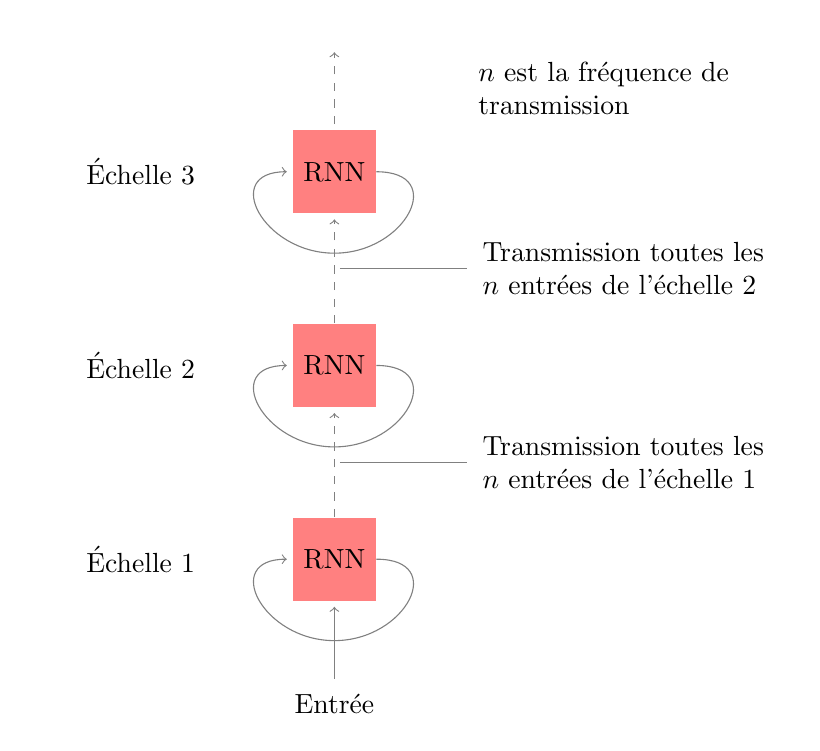
\begin{tikzpicture}[shorten >=2pt,->,draw=black!50, node distance=7em]
    \tikzstyle{every pin edge}=[<-,shorten <=2pt]
	\tikzstyle{module}=[minimum size=3em, fill=gray!50!]
	\tikzstyle{char}=[module, circle, fill=green!50!]
	\tikzstyle{text label}=[rectangle, text centered, text width=7.5em, node distance=7em]
	\tikzstyle{nn}=[rectangle, module, fill=orange!50!]
	\tikzstyle{rnn}=[nn, fill=red!50!]

	\node[rnn, pin={[pin edge={<-}, pin distance=3em]south:Entr\'{e}e}] (rnn1) {RNN};
	\node[rnn, above of=rnn1] (rnn2) {RNN};
	\node[rnn, above of=rnn2, pin={[pin edge={->,dashed}, pin distance=3em]north:}] (rnn3) {RNN};

	\foreach \n in {1,...,3}
		\draw[->] (rnn\n.east) to [out=0,in=0, looseness=2] ($(rnn\n.south) + (0,-.5)$) to [out=180,in=180, looseness=2] (rnn\n.west);

	\path[->,dashed] (rnn1)  edge coordinate (@aux) (rnn2);
	\path [late options={name=@aux, pin={[pin edge={-}, text width=10.5em, pin distance=5em]0:Transmission toutes les $n$ entr\'{e}es de l'\'{e}chelle 1}}];
	\path[->,dashed] (rnn2)  edge coordinate (@aux) (rnn3);
	\path [late options={name=@aux, pin={[pin edge={-}, text width=10.5em, pin distance=5em]0:Transmission toutes les $n$ entr\'{e}es de l'\'{e}chelle 2}}];

	\foreach \n in {1,...,3}
	    \node[text label, left of=rnn\n] (rnn\n l) {\'{E}chelle \n};
	\node[right of=rnn3, node distance=10.7em, text width=11em, yshift=3em] (rnn l) {$n$ est la fr\'{e}quence de transmission};
\end{tikzpicture}
	\caption[Principe de transmission de l'information d'une échelle à la suivante.]{Principe de transmission de l'information d'une échelle à la suivante. Ici, la fréquence de transmission est notée $n$.}
	\label{fig:gmsnn_transmit}
\end{figure}

Admettons que la capacité de mémoire d'un \gls{rnn} est de $9$ entrées (nombre arbitrairement défini pour l'exemple).
Si l'échelle supérieure récupère des informations toutes les $3$ entrées de la couche inférieure, ca capacité de mémoire devient $9*3=27$ entrées.
L'échelle encore au dessus aura une capacité mémoire de  $9*3*3=81$ entrées, et ainsi de suite.
Ici le nombre $3$ représente la fréquence à laquelle une échelle transmet des informations. On parlera par la suite de \og fréquence de transmission \fg{}.

\subsubsection{Plusieurs niveaux d'abstraction de l'information}
Une autre caractéristique importante du \gls{gmsnn} est qu'une échelle prend en entrée les informations abstraites par la couche précédente.
Ainsi, on peut s'attendre à ce que chaque échelle ajoute un niveau d'abstraction supplémentaire au modèle, comme sur la figure \ref{fig:gmsnn_ms}, \autopageref{fig:gmsnn_ms}.

\begin{figure}[ht]
	\centering
	\tikzstyle{tag} = [minimum height=1.5em, text width=5em, anchor=west]
\tikzstyle{tag2} = [minimum height=1.5em, text width=5em, anchor=east]
\tikzstyle{letter} = [draw, thin, fill=red!30, minimum height=1.5em, minimum width=1.5em]
\tikzstyle{module} = [rectangle, draw, thin, fill=green!30, minimum height=1.5em]
\tikzstyle{module-1} = [module, minimum width=1.5em]
\tikzstyle{module-2} = [module, minimum width=7.5em]
\tikzstyle{module-3} = [module, minimum width=25.5em]

    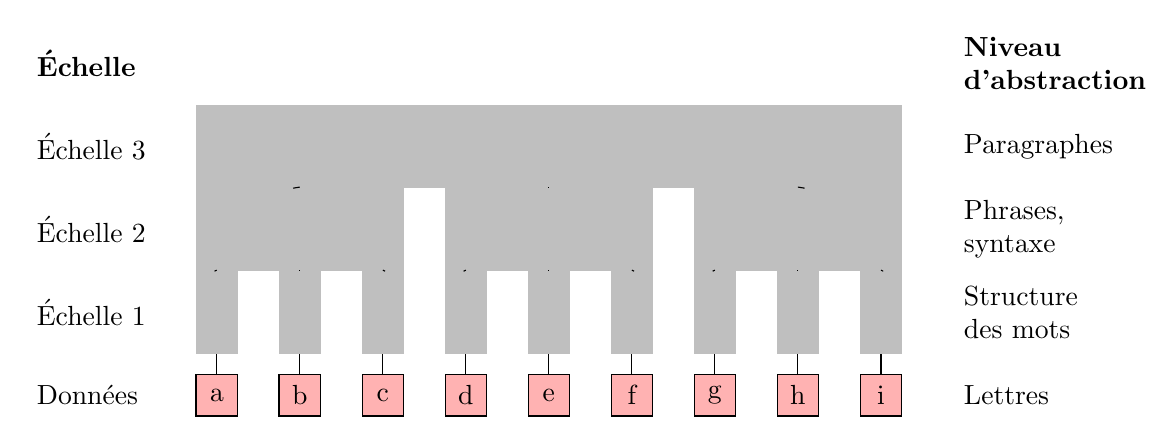
\begin{tikzpicture}[node distance=3em]
      \node[letter] (a) {a};
      \node[letter, right of=a] (b) {b};
      \node[letter, right of=b] (c) {c};
      \node[letter, right of=c] (d) {d};
      \node[letter, right of=d] (e) {e};
      \node[letter, right of=e] (f) {f};
      \node[letter, right of=f] (g) {g};
      \node[letter, right of=g] (h) {h};
      \node[letter, right of=h] (i) {i};
      
      \node[tag, right of=i, node distance=5.5em] (letters) {Lettres};
      \node[tag2, left of=a, node distance=4em] (e1) {Donn\'{e}es};
      
      \node[module-1, above of=a] (m-a) {};
      \node[module-1, above of=b] (m-b) {};
      \node[module-1, above of=c] (m-c) {};
      \node[module-1, above of=d] (m-d) {};
      \node[module-1, above of=e] (m-e) {};
      \node[module-1, above of=f] (m-f) {};
      \node[module-1, above of=g] (m-g) {};
      \node[module-1, above of=h] (m-h) {};
      \node[module-1, above of=i] (m-i) {};
      
      \node[tag, right of=m-i, node distance=5.5em] (word) {Structure des mots};
      \node[tag2, left of=m-a, node distance=4em] (e1) {\'{E}chelle 1};
      
      \node[module-2, above of=m-b] (m-abc) {};
      \node[module-2, above of=m-e] (m-def) {};
      \node[module-2, above of=m-h] (m-ghi) {};
      
      \node[tag, right of=m-ghi, node distance=8.5em] (sentence) {Phrases, syntaxe};
      \node[tag2, left of=m-abc, node distance=7em] (e2) {\'{E}chelle 2};
      
      \node[module-3, above of=m-def] (m-) {};
      
      \node[tag, right of=m-, node distance=17.5em] (paragraph) {Paragraphes};
      \node[tag2, left of=m-, node distance=16em] (e3) {\'{E}chelle 3};
      \node[tag, above of=paragraph, text width=5.9em, xshift=.45em, font=\bfseries] {Niveau d'abstraction};
      \node[tag2, above of=e3, font=\bfseries] {\'{E}chelle};
      
      \foreach \source / \target in {a/abc,b/abc,c/abc,d/def,e/def,f/def,g/ghi,h/ghi,i/ghi,abc/,def/,ghi/}
	      \path (m-\source.north) edge (m-\target);
	  \foreach \source / \target in {a,...,i} \path (\source.north) edge (m-\target);
    \end{tikzpicture}
	\caption[Différentes échelles, et les niveaux d'abstraction correspondants.]{%
		Différentes échelles, et les niveaux d'abstraction que l'on pourait attendre de celles-ci.
		Chaque bloc vert correspond à une entrée pour l'échelle correspondante.
		Les blocs bleus en bas du graphique correspond aux caractères qui sont fourni en entrée au modèle.
		Ici la fréquence de transmission vaut 3.}
	\label{fig:gmsnn_ms}
\end{figure}

\subsection{Adapter le modèle au volume de données et croissance du modèle}
Une propriété de l'architecture dérivée du principe d'échelles est de s'adapter au nombre d'entrées.

En effet, comme décrit dans la \autoref{subsec:scaling}, \autopageref{subsec:scaling}, le nombre d'échelles est dépendant du nombre d'entrées totales. 

On peut considérer que tant que aucune entrés ne lui est fournie, une échelle reste dans son état initial, elle n'\og existe\fg{} pas~; par conséquent, les échelles qui en sont dépendantes n'\og existent\fg{} pas non plus.

Ainsi, au fur et à mesure de l'entraînement, le modèle croit.

Il existe une formule pour déterminer le nombre de couches \og existantes\fg{} en fonction du nombre d'entrées présentées et de la fréquence de transmission~:

\[n = \lfloor\log_f i\rfloor + 1\]%
\[n: \text{nombre de couches}, i: \text{nombre d'entrées}, f: \text{fréquence de transmission}\]\label{growth_formula}

\subsubsection{Croissance potentiellement infinie du modèle}\label{inf_growth}
%[secondaire] la croissance: le modèle s'adapte au fur et à mesure que l'on lui fournit des données; plus exacte
Il est envisageable d'adapter le modèle au nombre d'entrées \textit{durant l'entraînement}, en créant réellement les échelles au fur et à mesure que l’on fournit les données.

Dans ce cas, tant que l'on lui fournit des données, la croissance du modèle est potentiellement infinie.

Comme décrit dans la \autoref{subsec:addcat_}, \autopageref{subsec:addcat_}, cette propriété à été abandonnée.

% TODO faire le schema
%\section{Architecture complète, des données aux prédictions}
%
%\begin{figure}[h]
%	\centering
%	\usetikzlibrary{calc}

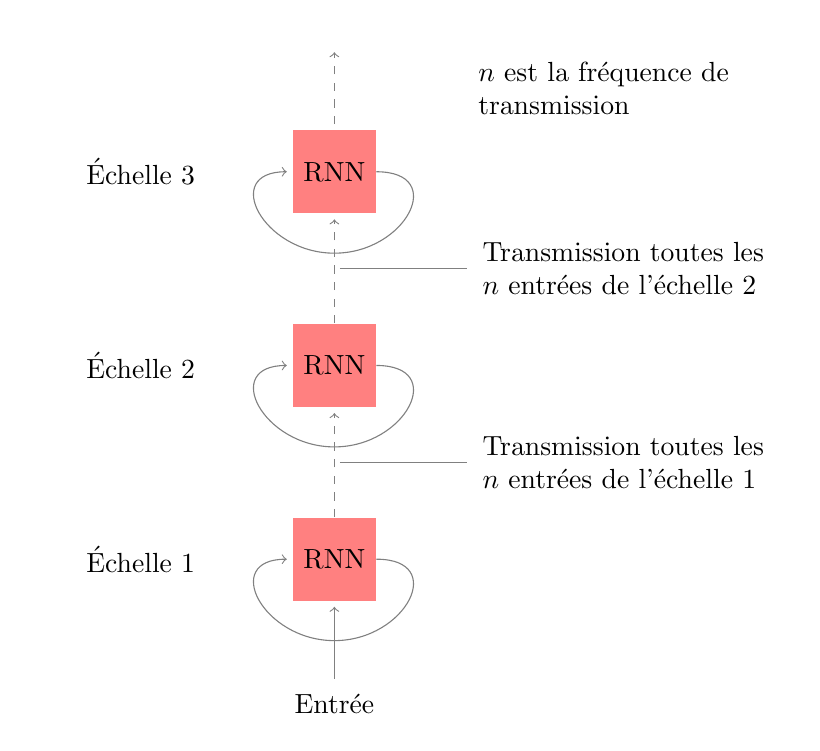
\begin{tikzpicture}[shorten >=2pt,->,draw=black!50, node distance=7em]
    \tikzstyle{every pin edge}=[<-,shorten <=2pt]
	\tikzstyle{module}=[minimum size=3em, fill=gray!50!]
	\tikzstyle{char}=[module, circle, fill=green!50!]
	\tikzstyle{text label}=[rectangle, text centered, text width=7.5em, node distance=7em]
	\tikzstyle{nn}=[rectangle, module, fill=orange!50!]
	\tikzstyle{rnn}=[nn, fill=red!50!]

	\node[rnn, pin={[pin edge={<-}, pin distance=3em]south:Entr\'{e}e}] (rnn1) {RNN};
	\node[rnn, above of=rnn1] (rnn2) {RNN};
	\node[rnn, above of=rnn2, pin={[pin edge={->,dashed}, pin distance=3em]north:}] (rnn3) {RNN};

	\foreach \n in {1,...,3}
		\draw[->] (rnn\n.east) to [out=0,in=0, looseness=2] ($(rnn\n.south) + (0,-.5)$) to [out=180,in=180, looseness=2] (rnn\n.west);

	\path[->,dashed] (rnn1)  edge coordinate (@aux) (rnn2);
	\path [late options={name=@aux, pin={[pin edge={-}, text width=10.5em, pin distance=5em]0:Transmission toutes les $n$ entr\'{e}es de l'\'{e}chelle 1}}];
	\path[->,dashed] (rnn2)  edge coordinate (@aux) (rnn3);
	\path [late options={name=@aux, pin={[pin edge={-}, text width=10.5em, pin distance=5em]0:Transmission toutes les $n$ entr\'{e}es de l'\'{e}chelle 2}}];

	\foreach \n in {1,...,3}
	    \node[text label, left of=rnn\n] (rnn\n l) {\'{E}chelle \n};
	\node[right of=rnn3, node distance=10.7em, text width=11em, yshift=3em] (rnn l) {$n$ est la fr\'{e}quence de transmission};
\end{tikzpicture}
%	\label{fig:gmsnn_model}
%	\caption[Architecture complète, des données aux prédictions]{Architecture complète du modèle \gls{gmsnn}, depuis les données jusqu'aux prédictions.
%	Ici, la fréquence de transmission}
%\end{figure}
}